\section{Bibliography Review}
\label{sec:bibliography-review}

A bibliographical research was performed to determine the state of the art in the field of the project,
both in terms of the models and algorithms used as well as the chosen state and action spaces which perform best
with regard to simulating realistic, real-world market dynamics.
The search was made using the Web of Science repository, covering the last 5 years, with the following search key:

\begin{verbatim}
    (
        "reinforcement learning" OR "dynamic programming" OR
        "optimal control" OR "control theory" OR "machine learning"
    )
    AND
    (
        "market making" OR "market maker"
    )
\end{verbatim}

Initially, 64 references were selected and deemed relevant to the project, with 23 of them being selected for further analysis and effectively used in our analysis,
and 4 additional references being added to the list after the initial selection.
The references were selected based on their relevance to the project and tagged according to the following groups
(for each non-binary category, combinations of tags were allowed):

\begin{itemize}
    \item Type of data (simulated, real-time connections, and others);
    \item Chosen state space (vectors of bid-ask spreads, order imbalance, N-depth order books, and others);
    \item Chosen action space (limit orders, market orders, and others);
    \item Chosen Reward space (spread, volume, profit, and others);
    \item Algorithms used (Q-Learning, Deep Q-Learning, Actor-Critic, or others);
    \item Whether a multi-agent approach was used (dueling or market agents);
    \item If a model-free environment was used (model-based or model-free);
    \item Metrics used for comparison (Sharpe Ratio, PnL, and others).
    \item Finally, results were tagged by their benchmarks, that is, the strategies used for comparison.
\end{itemize}

\subsection{State, Action, and Reward Spaces}
\label{subsec:state-action-and-reward-spaces}
State-of-the-art references defined state spaces primarily based on market-level observations,
specifically top-of-book quotes and n-depth book levels which align well with the real-time data available to market-making agents~\cite{He2023, Bakshaev2020}.
Additionally, agent inventory was also a common feature, reflecting the importance of managing risk and liquidity in market-making strategies~\cite{Patel2018, Ganesh2019}.
Action spaces included mostly only one pair of quotes, with some references allowing the choice of multiple bid-ask levels.
Some references also used book levels as discrete action space variables.

\begin{figure}[H]
    \centering
    % graph: images/state_space.png
    \makebox[\textwidth][c]{%
        \begin{subfigure}{.5\textwidth}
            \centering
            \includegraphics[width=\textwidth]{images/reward_space}
            \caption{Tagged reward space function variables}
            \label{fig:figure3}
        \end{subfigure}
        \hspace{0.02\textwidth} % Adjust spacing between figures
        \begin{subfigure}{0.5\textwidth}
            \centering
            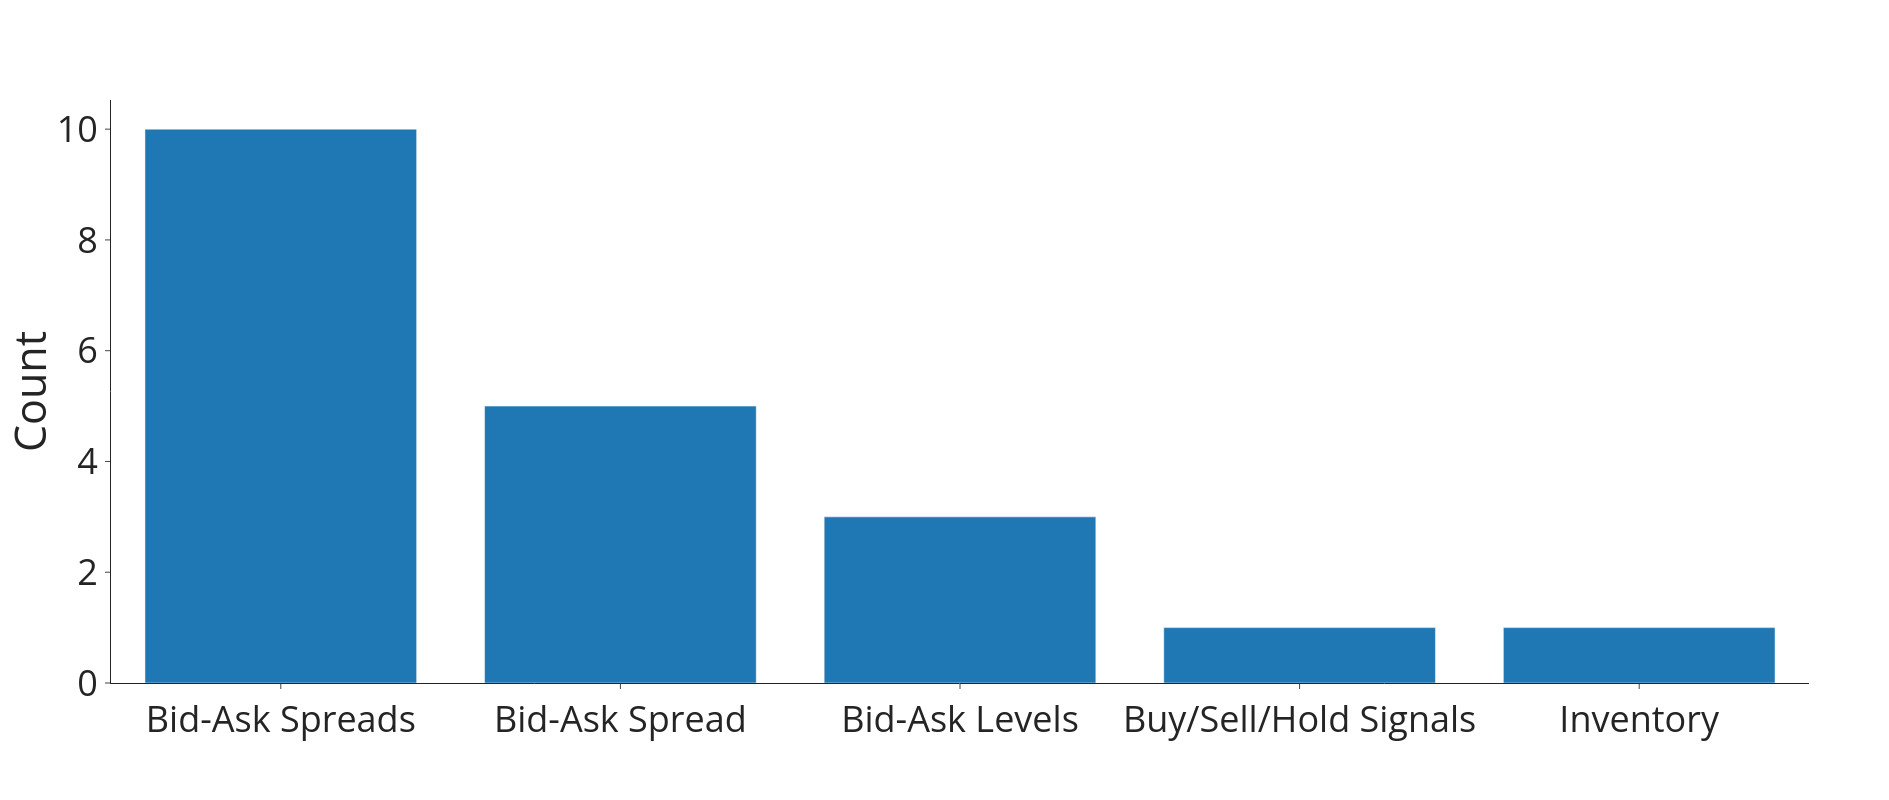
\includegraphics[width=\textwidth]{images/action_space}
            \caption{Tagged action space variables}
            \label{fig:figure2}
        \end{subfigure}
    }
    \centering
    % graph: images/state_space.png
    \makebox[\textwidth][c]{%
        \begin{subfigure}{0.7\textwidth}
            \centering
            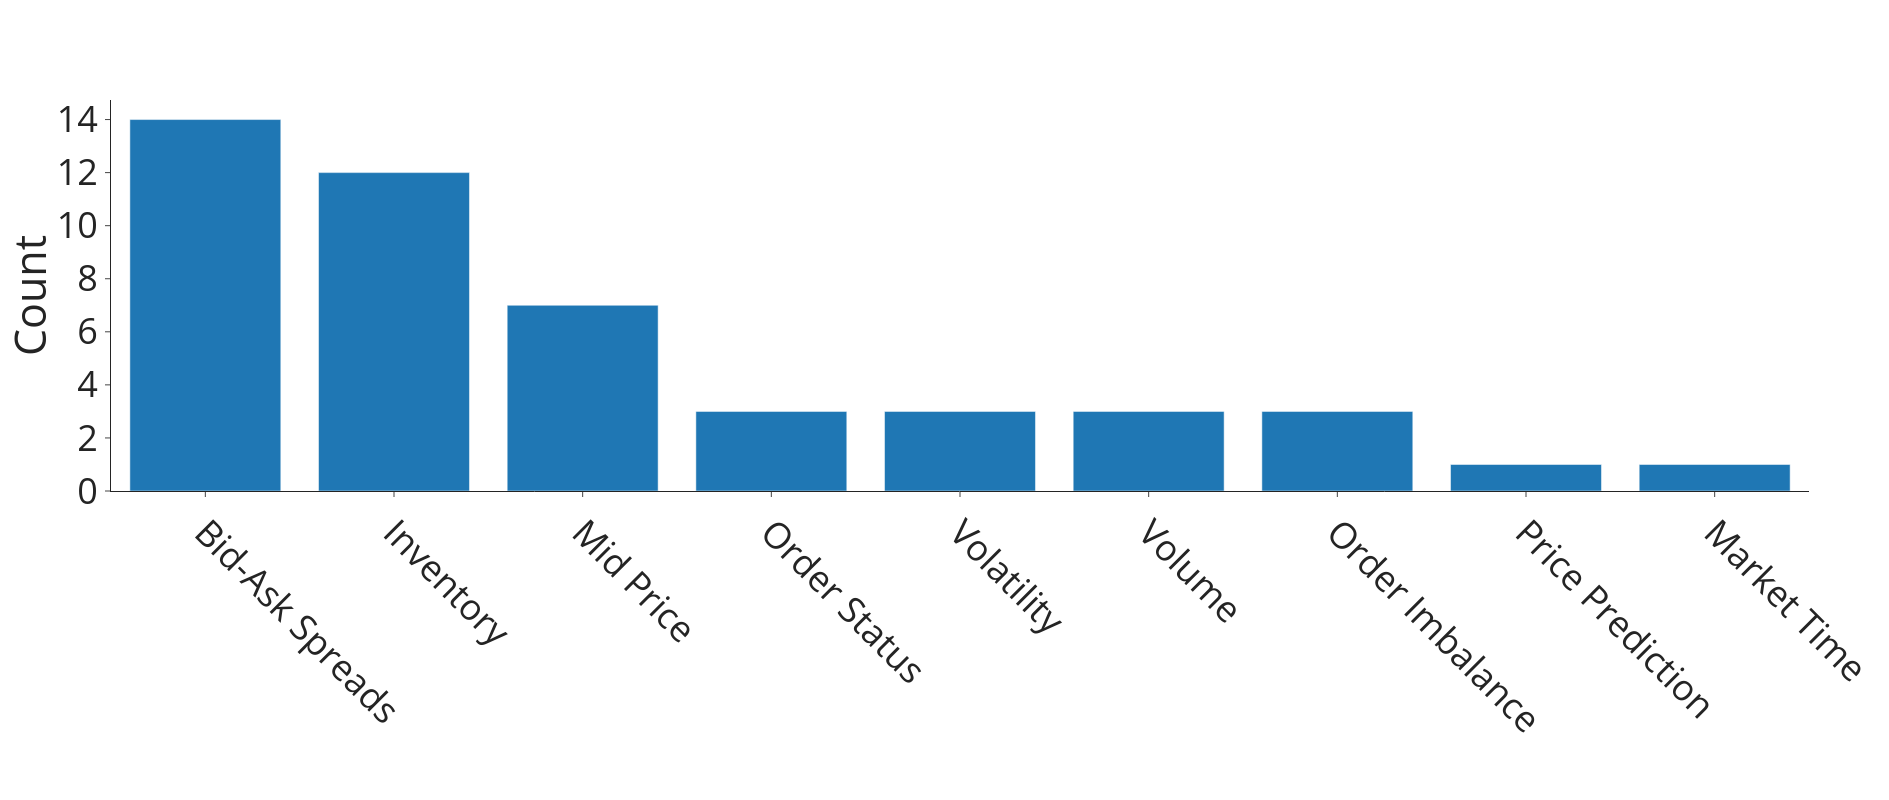
\includegraphics[width=\textwidth]{images/state_space}
            \caption{Taged state space variables}
            \label{fig:figure1}
        \end{subfigure}
    }
\end{figure}

Finally, almost all reward structures used some form of PnL and end-of-day or running liquidation and inventory penalties,
mostly due to the need to balance profitability and inventory risk~\cite{Sun2022, Gasperov2021}.
However, the inclusion of additional explicit constraints or reward penalties, such as inventory and overnight risk penalties was rarely discussed or mentioned,
even though being essential to ensure practical applicability and risk management in live trading scenarios~\cite{Jerome2022a, Selser2021a}.
The tagged action space variables include a separate ``Inventory`` variable that refeers to portfolio strategies that output a target maximum inventory.
For implementations that use specific quantities per order, no additional tags were used, as only one reference did not add quantities as part of the action space and instead used fixed quantities.

\subsection{Algorithms and Performance Metrics}
\label{subsec:algorithms-and-performance-metrics}
Recent trends in reinforcement learning research emphasize mostly model-free approaches, particularly Deep Q-Learning and Actor-Critic methods,
which leverage neural networks to approximate value functions or policies to deal with the high-dimensional nature of limit order books~\cite{Patel2018, Ganesh2019}.
The literature showed that model-free approaches had strong adaptability capabilities towards changing market conditions
while still maintaining acceptable training times, with PPO and DQN (and some DDQN) being the best performers in terms of convergence and stability~\cite{Sun2022, Gasperov2021a}.

\begin{figure}[H]
    \centering
    % graph: images/state_space.png
    \makebox[\textwidth][c]{%
        \begin{subfigure}{1\textwidth}
            \centering
            \includegraphics[width=\textwidth]{images/chosen_algorithms}
            \caption{Algorithms used as main research focus}
            \label{fig:figure4}
        \end{subfigure}
    }
\end{figure}

While market makers that maintain overnight positions obtain a worse long-term sharpe ratio compared to strategies that at end-of-day have null inventories,
the use of overnight position penalties was only mentioned in 3 of the references~\citep{Jerome2022a, Selser2021a, Sun2022}.

\begin{figure}[H]
    \centering
    % graph: images/state_space.png
    \makebox[\textwidth][c]{%
        \begin{subfigure}{.4\textwidth}
            \centering
            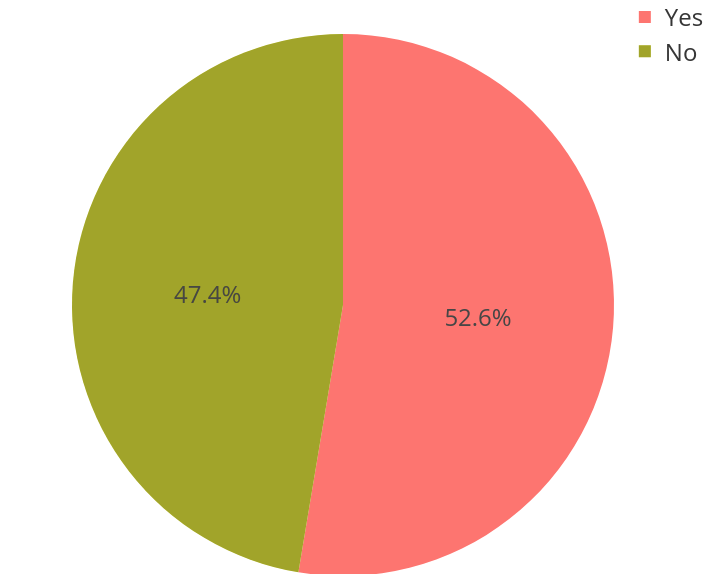
\includegraphics[width=\textwidth]{images/model_free}
            \caption{Principal algorithm is model free}
            \label{fig:figure5}
        \end{subfigure}
        \begin{subfigure}{.5\textwidth}
            \centering
            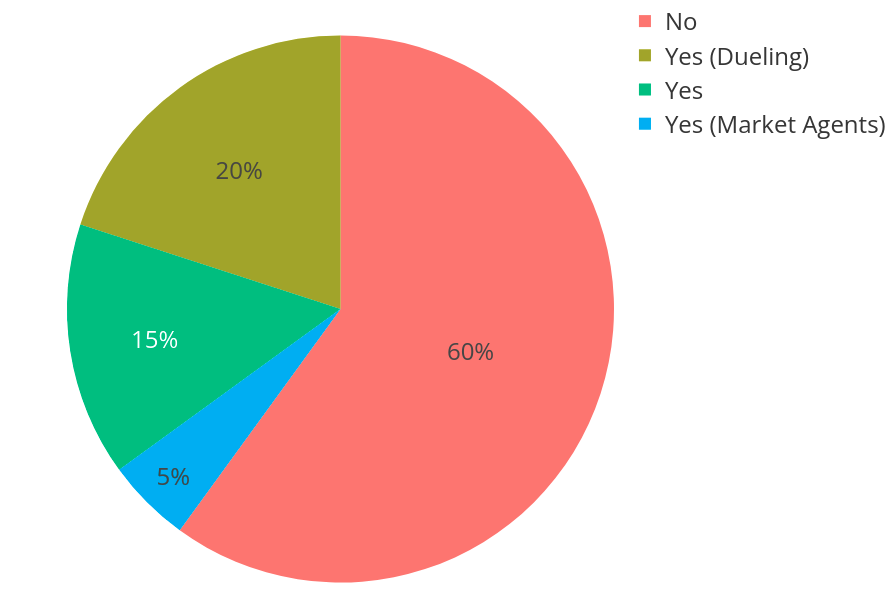
\includegraphics[width=\textwidth]{images/multi_agent}
            \caption{Multiple agents used in training}
            \label{fig:figure6}
        \end{subfigure}
    }
\end{figure}

Overall, the bibliographical review underscores the growing relevance and preference for reinforcement learning algorithms in the market-making domain,
particularly when combined with realistic state, action, and reward spaces.
The insights gained from the state and action spaces, as well as the reward function guided our choice for the space variables used in this paper,
as well as the design for our chosen neural network architecture,
while still showing a gap in the literature regarding usage of restrictions in the RL framework, both as hard limits and incentives.
